% =====================================================================
%  AI Invoice Auditor — Capstone Presentation (Overleaf / Beamer)
%  5 slides: Welcome | Infrastructure | Challenges | Beyond Scope | Thanks
%  Compile with pdfLaTeX on Overleaf.
% =====================================================================
\documentclass[aspectratio=169]{beamer}

\usetheme{Madrid}
\usecolortheme{whale}
\useinnertheme{circles}

\usepackage{tikz}
\usepackage{textcomp}
\usepackage{fontawesome5}
\usetikzlibrary{shapes.geometric, arrows.meta, positioning, calc, backgrounds, fit}

% ---- Colour palette --------------------------------------------------
\definecolor{brandblue}{RGB}{30,58,95}
\definecolor{accent}{RGB}{37,99,235}
\definecolor{softgrey}{RGB}{241,245,249}
\definecolor{good}{RGB}{21,128,61}
\definecolor{warn}{RGB}{180,83,9}
\definecolor{bad}{RGB}{185,28,28}
\definecolor{store}{RGB}{15,118,110}

\setbeamercolor{structure}{fg=brandblue}
\setbeamercolor{frametitle}{bg=brandblue,fg=white}
\setbeamertemplate{navigation symbols}{}
\setbeamertemplate{footline}[frame number]

% ---- TikZ node / edge styles -----------------------------------------
% NOTE: 'step' is a reserved TikZ key (grid step); we use 'proc' instead.
\tikzset{
  svc/.style   ={rectangle, rounded corners=3pt, draw=brandblue, very thick,
                 fill=white, text=brandblue, font=\scriptsize\bfseries,
                 minimum width=2.0cm, minimum height=0.95cm, align=center},
  db/.style    ={cylinder, shape border rotate=90, aspect=0.28, draw=store,
                 very thick, fill=store!12, text=store, font=\scriptsize\bfseries,
                 minimum width=1.9cm, minimum height=1.0cm, align=center},
  proc/.style  ={rectangle, rounded corners=2pt, draw=brandblue, thick,
                 fill=softgrey, text=brandblue, font=\scriptsize\bfseries,
                 minimum width=1.8cm, minimum height=0.8cm, align=center},
  dec/.style   ={diamond, aspect=1.7, draw=brandblue, very thick, fill=softgrey,
                 text=brandblue, font=\tiny\bfseries, align=center, inner sep=1pt,
                 minimum width=1.8cm, minimum height=1.25cm},
  term/.style  ={rectangle, rounded corners=10pt, draw=brandblue, thick,
                 fill=brandblue!15, text=brandblue, font=\scriptsize\bfseries,
                 minimum width=1.4cm, minimum height=0.65cm, align=center},
  flow/.style  ={-{Stealth[length=2.2mm]}, brandblue, thick},
  biflow/.style={{Stealth[length=2.2mm]}-{Stealth[length=2.2mm]}, store, thick},
  dash/.style  ={-{Stealth[length=2.2mm]}, accent, thick, dashed},
  lbl/.style   ={font=\tiny, text=brandblue!85, fill=white, inner sep=1.3pt,
                 rounded corners=1pt, align=center},
}

% =====================================================================
\begin{document}

% ---------------------------------------------------------------------
% SLIDE 1 — WELCOME
% ---------------------------------------------------------------------
{
\setbeamertemplate{footline}{}
\begin{frame}[plain]
  \begin{tikzpicture}[remember picture,overlay]
    \fill[brandblue] (current page.north west) rectangle (current page.south east);
    \fill[accent!85] (current page.south west) rectangle
        ([yshift=1.55cm]current page.south east);
  \end{tikzpicture}

  \vspace{0.9cm}
  \begin{center}
    {\color{white}\Huge\bfseries AI Invoice Auditor}\\[6pt]
    {\color{white!85}\Large A Containerized, Multilingual Invoice Validation System}\\[12pt]
    {\color{white!70}\normalsize
      Agentic AI \textbullet\ LangGraph \textbullet\ RAG \textbullet\ Human-in-the-Loop}\\[18pt]

    % {\color{white!80}\footnotesize
      % \faIcon{cubes}\ \ 6-Service Docker Stack \quad\textbullet\quad
      % \faIcon{language}\ \ EN / ES / DE \quad\textbullet\quad
      % \faIcon{database}\ \ Durable Audit Trail}
      \vspace{0.8cm}
  \end{center}

  \vfill
  \begin{center}
    {\color{white}\footnotesize\bfseries Group 11}\\[3pt]
    {\color{white!90}\footnotesize
      Anshuman Shukla (1458243) \quad Aman Patidar (1458242)}\\[2pt]
    {\color{white!90}\footnotesize
      Ayush Gupta (1458241) \quad Param Srivastava (1458240)}\\[8pt]
    {\color{white}\scriptsize Capstone Project — Batch Jul26-SP1-L2-Agentic-AI}
  \end{center}
  \vspace{0.5cm}
\end{frame}
}

% ---------------------------------------------------------------------
% SLIDE 2 — INFRASTRUCTURE / ARCHITECTURE
% ---------------------------------------------------------------------
\begin{frame}{Infrastructure \& Architecture}
  \centering
  % Six physical services only. Internal protocols are summarized inside Agent.
  % Horizontal service calls; separate downward paths to each store.
  \resizebox{0.95\linewidth}{!}{%
  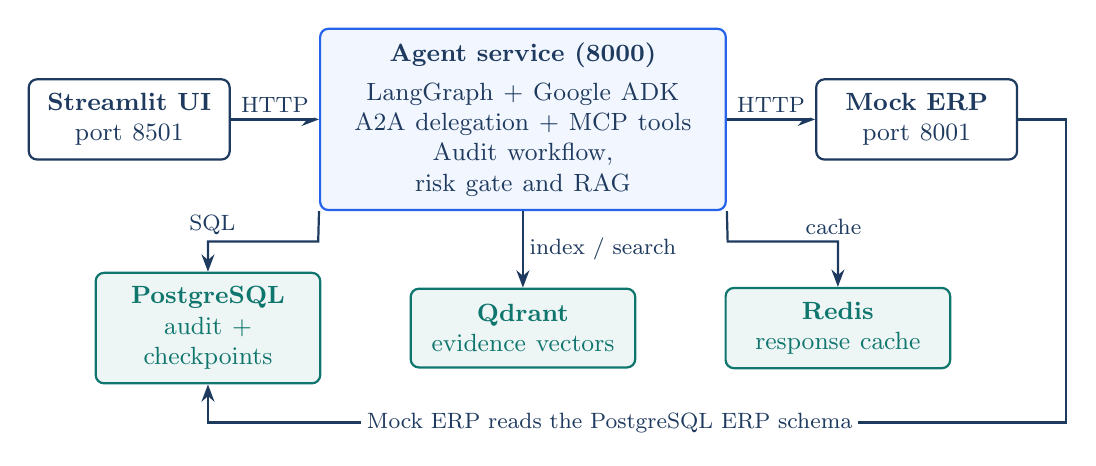
\begin{tikzpicture}[
    cleanservice/.style={rectangle,rounded corners=3pt,draw=brandblue,thick,
      fill=white,text=brandblue,font=\small\bfseries,align=center,
      text width=2.2cm,minimum height=1.0cm,inner sep=5pt},
    cleanstore/.style={cleanservice,draw=store,fill=store!7,text=store,
      text width=2.5cm},
    cleanlabel/.style={font=\footnotesize,text=brandblue,fill=white,
      inner sep=2pt,align=center}
  ]
    % Row 1: user interface, orchestration and ERP service.
    \node[cleanservice] (cui) at (0,2.3) {Streamlit UI\\\normalfont port 8501};
    \node[cleanservice,text width=4.8cm,minimum height=1.65cm,
      fill=accent!6,draw=accent] (cagent) at (5,2.3)
      {Agent service (8000)\\[3pt]
       \normalfont LangGraph + Google ADK\\
       A2A delegation + MCP tools\\
       Audit workflow, risk gate and RAG};
    \node[cleanservice] (cerp) at (10,2.3)
      {Mock ERP\\\normalfont port 8001};

    \draw[flow] (cui)--(cagent) node[cleanlabel,midway,above]{HTTP};
    \draw[flow] (cagent)--(cerp) node[cleanlabel,midway,above]{HTTP};

    % Row 2: three independent data responsibilities.
    \node[cleanstore] (cpg) at (1,-0.35)
      {PostgreSQL\\\normalfont audit + checkpoints};
    \node[cleanstore] (cqd) at (5,-0.35)
      {Qdrant\\\normalfont evidence vectors};
    \node[cleanstore] (crd) at (9,-0.35)
      {Redis\\\normalfont response cache};

    \draw[flow] (cagent.south west) -- (2.4,0.75) -| (cpg.north)
      node[cleanlabel,pos=0.48,above]{SQL};
    \draw[flow] (cagent.south)--(cqd.north)
      node[cleanlabel,midway,right]{index / search};
    \draw[flow] (cagent.south east) -- (7.6,0.75) -| (crd.north)
      node[cleanlabel,pos=0.48,above]{cache};

    % ERP SQL stays outside the other connectors; no crossing through nodes.
    \draw[flow] (cerp.east) -- (11.9,2.3) -- (11.9,-1.55)
      -- (1,-1.55) -- (cpg.south);
    \node[cleanlabel] at (6.1,-1.55) {Mock ERP reads the PostgreSQL ERP schema};
  \end{tikzpicture}}

  \vspace{3mm}
  {\small\textbf{Added layers:} ADK/A2A interoperability, MCP discovery,
  Responsible AI controls and Langfuse tracing.}\par
  \vspace{1mm}
  {\footnotesize Six services share \texttt{auditor\_net}.
  MCP/A2A dispatch is in-process by default; Langfuse is external.}
\end{frame}

% ---------------------------------------------------------------------
% SLIDE 3 — CHALLENGES FACED
% ---------------------------------------------------------------------
\begin{frame}{Challenges Faced}
  \small
  \renewcommand{\arraystretch}{1.38}
  \setlength{\tabcolsep}{5pt}
  \begin{tabular}{@{}p{3.3cm}p{10.1cm}@{}}
    \textbf{\color{brandblue}Challenge} &
    \textbf{\color{brandblue}Approach in the current system} \\ \hline
    \textbf{Cross-framework coordination} &
    Delegate translation and business-validation skills through A2A;
    return structured task results and expose the actual executor. \\
    \textbf{Consistent tool access} &
    Register shared capabilities with MCP metadata;
    discover tools by name and return consistent results/errors. \\
    \textbf{Unsafe input and limited visibility} &
    Apply RAI checks to relevant input/output boundaries;
    use Langfuse traces and nested spans to inspect errors and fallbacks. \\
    \textbf{Premature knowledge indexing} &
    Add a risk gate: low-risk invoices auto-index;
    pending cases wait for a reviewer to approve or reject. \\ \hline
  \end{tabular}

  \vspace{4mm}
  {\color{brandblue}\textbf{Normal processing route}}\par
  \vspace{1mm}
  Report $\to$ Risk gate $\to$
  \textcolor{good}{Auto-approved: index}
  \quad / \quad
  \textcolor{warn}{Pending: human review}

  \vspace{3mm}
  {\footnotesize Existing extraction, ERP validation and RAG remain the baseline.
  These changes add coordination, safety and execution visibility.}
\end{frame}

% ---------------------------------------------------------------------
% SLIDE 4 — APPROACHES BEYOND SCOPE (Human-in-the-Loop)
% ---------------------------------------------------------------------
\begin{frame}{Beyond Scope --- Human-in-the-Loop Review}
  \begin{columns}[T]

  % LEFT: HITL diagram (matches the designed revalidation loop)
  \begin{column}{0.55\textwidth}
  \centering
  \resizebox{!}{0.80\textheight}{%
  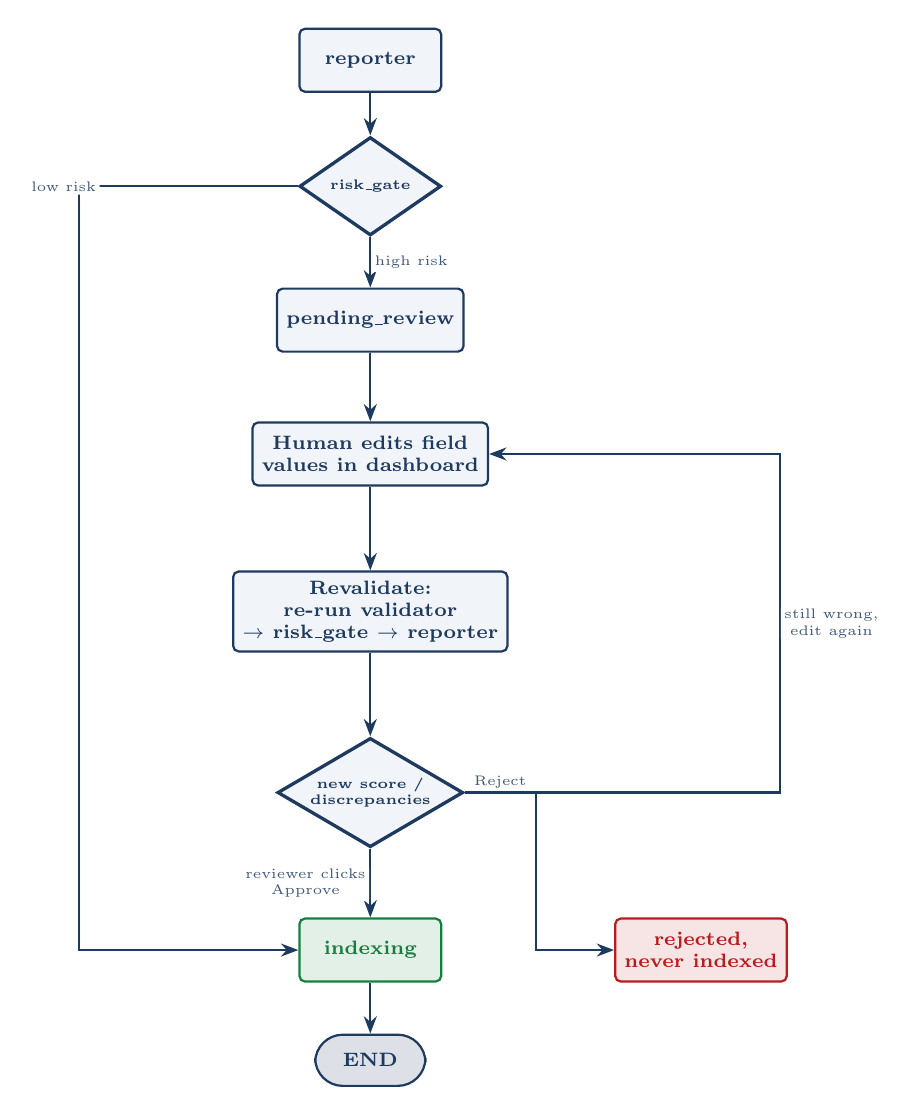
\begin{tikzpicture}
    \node[proc]  (rep)   at (0,0)     {reporter};
    \node[dec]   (gate)  at (0,-1.6)  {risk\_gate};
    \node[proc]  (pend)  at (0,-3.3)  {pending\_review};
    \node[proc]  (edit)  at (0,-5.0)  {Human edits field\\values in dashboard};
    \node[proc]  (reval) at (0,-7.0)  {Revalidate:\\re-run validator\\$\to$ risk\_gate $\to$ reporter};
    \node[dec]   (score) at (0,-9.3)  {new score /\\discrepancies};
    \node[proc, fill=good!12, draw=good, text=good] (idxn) at (0,-11.3) {indexing};
    \node[term]  (end)   at (0,-12.7) {END};
    \node[proc, fill=bad!12, draw=bad, text=bad] (rej) at (4.2,-11.3) {rejected,\\never indexed};

    % main chain
    \draw[flow] (rep)--(gate);
    \draw[flow] (gate)--(pend) node[lbl,pos=0.5,right]{high risk};
    \draw[flow] (pend)--(edit);
    \draw[flow] (edit)--(reval);
    \draw[flow] (reval)--(score);
    \draw[flow] (idxn)--(end);

    % low-risk bypass (far left) into indexing
    \draw[flow] (gate.west) -- (-3.7,-1.6) node[lbl,pos=0.9,left]{low risk}
                -- (-3.7,-11.3) -- (idxn.west);

    % approve / reject / loop out of the score decision
    \draw[flow] (score)--(idxn) node[lbl,pos=0.5,left]{reviewer clicks\\Approve};
    \draw[flow] (score.east) -- (2.1,-9.3) node[lbl,pos=0.5,above]{Reject} |- (rej.west);
    \draw[flow] (score.east) -- (5.2,-9.3) -- (5.2,-5.0) node[lbl,pos=0.5,right]{still wrong,\\edit again} -- (edit.east);
  \end{tikzpicture}}
  \end{column}

  % RIGHT: bullets (flat list to guarantee fit)
  \begin{column}{0.45\textwidth}
  \footnotesize
  \textbf{\color{brandblue}A real revalidation loop (not required by spec)}
  \begin{itemize}\setlength\itemsep{4pt}
    \item \textbf{risk\_gate} scores every invoice: \textbf{low risk} auto-indexes; \textbf{high risk} is held as \texttt{pending\_review}
    \item Auditor \textbf{clicks into} a held invoice and \textbf{edits field values \& line items}
    \item \textbf{Revalidate} re-runs \texttt{validator $\to$ risk\_gate $\to$ reporter}, returning a \textbf{new score / discrepancies}
    \item \textbf{Approve} $\to$ indexed into Qdrant; \textbf{Reject} $\to$ never indexed; \textbf{still wrong} $\to$ edit again (loop)
    \item Edits stored \textbf{immutably} in \texttt{audit.human\_feedback} --- original extraction never overwritten
  \end{itemize}
  \emph{\scriptsize APIs: \texttt{/review/queue} \textbullet\ \texttt{/revalidate} \textbullet\ \texttt{/approve} \textbullet\ \texttt{/reject}}
  \end{column}
  \end{columns}
\end{frame}

% ---------------------------------------------------------------------
% SLIDE 5 — THANK YOU (with team split)
% ---------------------------------------------------------------------
{
\setbeamertemplate{footline}{}
\begin{frame}[plain]
  \begin{tikzpicture}[remember picture,overlay]
    \fill[brandblue] (current page.north west) rectangle (current page.south east);
  \end{tikzpicture}

  \vfill
  \begin{center}
    {\color{white}\fontsize{60}{66}\selectfont\bfseries Thank You!}
  \end{center}
  \vfill
\end{frame}
}

\end{document}
